\chapter{Baseline Evaluation Results}
\label{ch:baseline_evaluation_results}
This chapter presents the baseline evaluation results for CloudSentinel in the Online Boutique environment. It describes the onboarding work, two completed CPU-stress scenarios, and the limitations that became visible during their execution. Chapter~8 evaluates these findings against the criteria defined in Chapter~5.

\section{Online Boutique: onboarding and operationalisation}
Online Boutique was the first application on which CloudSentinel was configured outside the original SMD and Sock Shop settings. The case shows that CloudSentinel can be connected to a Prometheus-monitored Kubernetes application, but that this requires application-specific configuration and data preparation.

\subsection{Deployment and connectivity}
CloudSentinel was deployed using the provided Kubernetes manifests. Prometheus was deployed through the \texttt{prometheus-community} Helm chart. To connect CloudSentinel to the monitoring stack, the Prometheus endpoint was configured manually through the CloudSentinel interface. In this deployment, the endpoint was \texttt{http://127.0.0.1:55725}.

An additional namespace change was required. The \texttt{CLUSTER\_NAMESPACE} value in the monitoring deployment configuration was changed from \texttt{cloudsentinel} to \texttt{default}, because Online Boutique was deployed in the default namespace. Without this change, CloudSentinel could not identify the relevant application pods.

\subsection{Metric selection and data preparation}
CloudSentinel's original datasets and examples could not be used directly for Online Boutique. Relevant Prometheus metrics were selected and aggregated at pod level: CPU usage, CPU throttling, memory usage, and pod restart rate. The load-generator pod was excluded because it generated workload rather than representing an application component to be monitored.

The selected series were exported from Prometheus and prepared with custom scripts. This required selecting relevant entities, aligning timestamps, reshaping the metric data into CloudSentinel's expected arrays, constructing normal-behaviour training data, constructing testing data that included fault periods, and creating labels from the recorded fault intervals. These activities were necessary before a model could be trained or a scenario could be analysed.

\subsection{Configuration and manual intervention}
Several configuration and operational steps required manual intervention. In addition to the Prometheus endpoint and namespace changes, metric mappings had to be defined for Online Boutique. The model trained on the selected baseline data also had to be made available to the live-monitoring workflow. Configuration changes made through the interface did not always propagate automatically to the components that performed monitoring or inference, requiring additional checking and manual correction.

These observations show that CloudSentinel can be configured for a new environment, but that the process is not yet a self-contained or reproducible onboarding workflow.

\subsection{Summary of onboarding effort}
Table~\ref{tab:online_boutique_onboarding} summarises the main onboarding activities. The table records practical effort rather than precise time measurements, as the setup process was iterative and included troubleshooting.

\begin{table}[htbp]
    \centering
    \small
    \caption{Main onboarding activities for Online Boutique.}
    \label{tab:online_boutique_onboarding}
    \begin{tabular}{p{0.28\textwidth} p{0.30\textwidth} p{0.30\textwidth}}
        \toprule
        \textbf{Activity} & \textbf{Artefact or configuration} & \textbf{Observed friction} \\
        \midrule
        Deploy framework and monitoring stack & Kubernetes manifests and Prometheus Helm chart & Components had to be configured separately. \\
        Configure monitoring access & Prometheus endpoint and namespace setting & Default namespace configuration did not match Online Boutique. \\
        Select and map metrics & Prometheus queries and pod-level feature set & Original examples did not match Online Boutique services or labels. \\
        Prepare datasets & Custom export, alignment, reshaping, and labelling scripts & Manual work was needed to construct training, testing, and label arrays. \\
        Configure live workflow & Trained model and monitoring configuration & Configuration propagation required manual checking and correction. \\
        \bottomrule
    \end{tabular}
\end{table}

\section{Online Boutique: end-to-end workflow under controlled interventions}
This section presents the anomaly detection and RCA results from the controlled CPU-stress scenarios in Online Boutique. Each scenario is reported as one end-to-end workflow: the fault injection, the live-monitoring output, RCA triggering, the RCA ranking, and the manual replay results are discussed together.

\subsection{Interpreting the CloudSentinel monitoring output}
Two related workflows were used. First, live monitoring was used to assess whether CloudSentinel could operate in the deployed environment. It repeatedly retrieved recent Prometheus data, calculated an anomaly percentage, and triggered RCA when that percentage exceeded the configured RCA threshold.

Second, historical Prometheus data were exported and processed after the experiment. This is referred to as \textit{manual replay}. Manual replay produced one anomaly prediction per scoreable timestamp. Since the fault interval was recorded during the experiment, these predictions could be compared with manually created labels. This made it possible to inspect true positives, false positives, true negatives, false negatives, precision, recall, and F1-score.

CloudSentinel uses a forecasting-based detector. For each scoreable timestamp, the detector uses the preceding lookback window as input and predicts the following metric values. The difference between the predicted and observed values is used as an anomaly score. A saved value called \texttt{epsilon} is used as the anomaly threshold. A timestamp is classified as anomalous when its global anomaly score is greater than or equal to this threshold.

The percentage shown in the live-monitoring graph is the proportion of scoreable timestamps in the current monitoring iteration that are classified as anomalous. For example, a value of 14.286\% means that 14.286\% of the scoreable timestamps in that iteration crossed the stored anomaly threshold. RCA is triggered when this percentage is greater than the configured RCA threshold.

The number of scoreable timestamps is smaller than the number of input timestamps because the first part of an input window is used as lookback context. With the configured lookback of 100 timestamps, CloudSentinel cannot produce a prediction for the first 100 timestamps in a submitted dataset or monitoring window.

The live and manual workflows are related but not identical. During training, the data-processing component fits a Min--Max scaler to the training data and uses that same scaler to transform the accompanying test data. During a detection-only request, however, the implementation fits a new Min--Max scaler to the submitted data. Since live monitoring repeatedly submits recent monitoring windows, the scaling range can differ between monitoring iterations. This limitation is important when interpreting the live and manual results below.

\subsection{Single-pod CPU stress on \texttt{paymentservice}}
\subsubsection{Fault injection and setup}
This scenario examined whether CloudSentinel could detect CPU pressure affecting one service pod and whether the subsequent RCA output would identify \texttt{paymentservice} or its related metrics as relevant candidates.

Table~\ref{tab:paymentservice-cpu-setup} summarises the scenario configuration.

\begin{table}[htbp]
    \centering
    \small
    \caption{Configuration of the single-pod CPU-stress scenario.}
    \label{tab:paymentservice-cpu-setup}
    \begin{tabular}{l l}
        \toprule
        \textbf{Item} & \textbf{Value} \\
        \midrule
        Target component & \texttt{paymentservice} \\
        Fault mechanism & CPU-intensive \texttt{yes} process in an ephemeral debug container \\
        Fault start & 15:20 UTC (17:20 local time) \\
        Fault end & 15:45 UTC (17:45 local time) \\
        Monitoring data window & 16:35--18:15 local time \\
        Live-monitoring duration & 30 minutes \\
        \bottomrule
    \end{tabular}
\end{table}

The fault was injected by starting a CPU-intensive \texttt{yes} process in an ephemeral BusyBox debug container attached to the \texttt{paymentservice} pod. The process continuously consumed CPU resources. The \texttt{wait} command kept the shell session active until the process was terminated.

\begin{verbatim}
kubectl debug pod/paymentservice -it --image=busybox:1.36 \
-- sh -c 'yes > /dev/null & wait'
\end{verbatim}

\subsubsection{Live-monitoring result}
Figure~\ref{fig:paymentservice-cpu-live} shows the live anomaly percentage during the CPU-stress injection. The percentage increased shortly after the stress process was started, crossed the configured 4\% RCA threshold several times, and decreased after the process was stopped. This shows that the live workflow responded to the intervention: Prometheus data were collected, CloudSentinel produced an anomaly percentage, the threshold triggered RCA, and RCA output was displayed.

A temporary dip was visible around 17:31 local time while the CPU-stress process was still active. Therefore, the graph should not be read as a direct timestamp-level measure of fault severity. A likely explanation is discussed in the interpretation of the scenario.

\begin{figure}[htbp]
    \centering
    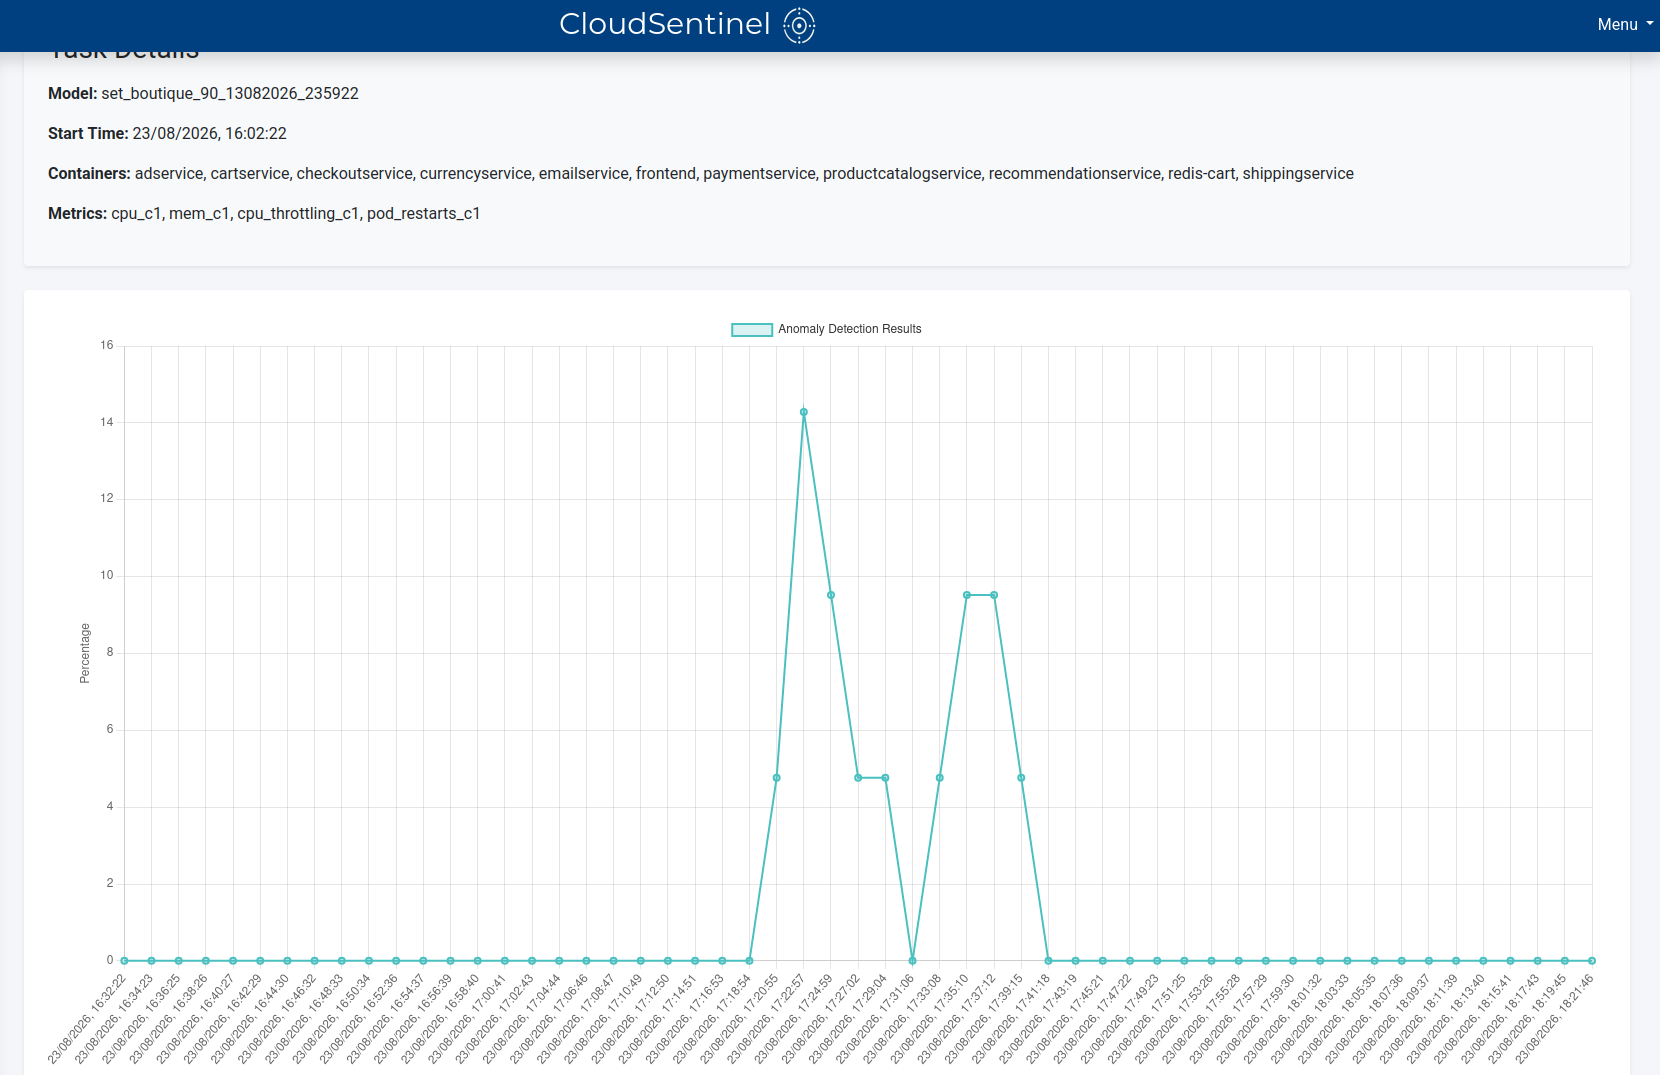
\includegraphics[width=\textwidth]{figures/boutique/scenario1/live_monitoring_graph_data.png}
    \caption{CloudSentinel live-monitoring view during CPU stress injected into \texttt{paymentservice}. The fault was active from 17:20 to 17:45 local time. The graph displays the percentage of scoreable timestamps classified as anomalous in each monitoring iteration.}
    \label{fig:paymentservice-cpu-live}
\end{figure}

A UI-related issue was observed during this session. Live monitoring was started at approximately 16:35 local time, but the interface displayed a session timestamp of 16:02:22. The displayed time therefore appeared to be offset by approximately the configured 30-minute monitoring duration. Interface timestamps could not be directly interpreted as actual execution times without manually comparing them with the recorded fault-injection times.

\subsubsection{RCA result}
RCA was triggered nine times during the session. These events corresponded to the nine displayed anomaly percentages above the 4\% RCA threshold. The first RCA execution occurred at approximately 17:20 local time, shortly after the CPU-stress injection started, and was associated with an anomaly percentage of 4.762\%. In the interface dropdown, however, this event was displayed with timestamp 16:50:55, again indicating an offset close to the configured monitoring duration.

The first RCA ranking partly represented the affected component. \texttt{paymentservice\_cpu\_throttling\_c1} ranked second and \texttt{paymentservice\_mem\_c1} ranked third. Direct CPU usage for \texttt{paymentservice}, however, ranked only 26th. The highest-ranked metric was \texttt{currencyservice\_cpu\_c1}, rather than a \texttt{paymentservice}-related metric.

The highest anomaly percentage observed during the session was 14.286\%. Despite this stronger anomaly signal, the corresponding RCA ranking represented \texttt{paymentservice} less clearly. The relevant pod-restart, CPU, CPU-throttling, and memory metrics ranked between positions 22 and 34.

Table~\ref{tab:paymentservice-cpu-rca} summarises three representative RCA events: the first trigger, the event with the highest anomaly percentage, and the final observed trigger.

\begin{table}[htbp]
    \centering
    \scriptsize
    \caption{Selected RCA results during single-pod CPU stress on \texttt{paymentservice}.}
    \label{tab:paymentservice-cpu-rca}
    \begin{tabularx}{\textwidth}{l c X X}
        \toprule
        \textbf{RCA event} & \textbf{Anomaly percentage} & \textbf{Relevant \texttt{paymentservice} output} & \textbf{Interpretation} \\
        \midrule
        First RCA trigger
        & 4.762\%
        & CPU throttling: rank 2, score 0.08084; memory: rank 3, score 0.03491; pod restarts: rank 21; CPU: rank 26, score 0.02622
        & Some relevant metrics were ranked prominently, but direct CPU usage was low-ranked. \\

        Highest anomaly trigger
        & 14.286\%
        & Pod restarts: rank 22, score 0.02701; CPU: rank 29, score 0.02260; CPU throttling: rank 30, score 0.01838; memory: rank 34, score 0.01222
        & The affected service was weakly represented despite the strongest observed anomaly percentage. \\

        Last observed RCA trigger
        & Not recorded separately
        & Pod restarts: rank 26; memory: rank 27; CPU: rank 29; CPU throttling: rank 31
        & Relevant metrics were low-ranked; RCA did not reliably localise the affected component. \\
        \bottomrule
    \end{tabularx}
\end{table}

\subsubsection{Manual replay result}
The manual evaluation was performed in two stages. First, the exported historical metric data were processed through the CloudSentinel manual detection workflow. This workflow generated point-level output in \texttt{scenario\_prediction\_output.csv}, including a global anomaly score and a binary anomaly prediction for each scoreable timestamp.

Second, \texttt{calculate\_stats.py} compared these binary predictions with ground-truth labels derived from the recorded CPU-stress interval. The script aligned the prediction output with the corresponding labels before calculating true positives, false positives, true negatives, and false negatives. Precision, recall, and F1-score were then calculated from these aligned values.

The input data contained 381 timestamps. Because the model used a lookback of 100 timestamps, manual detection generated 281 aligned output predictions. Within this aligned window, 101 timestamps were labelled as part of the CPU-stress interval and 180 timestamps were labelled as normal operation.

The stored threshold was evaluated first. Lower thresholds were then examined as exploratory sensitivity analysis. For each threshold setting, the same model, input data, ground-truth labels, and alignment procedure were retained; only the value used to convert the global anomaly score into a binary prediction was changed.

Table~\ref{tab:paymentservice-cpu-manual} summarises the manual replay results.

\begin{table}[htbp]
    \centering
    \small
    \caption{Exploratory manual replay results for the single-pod CPU-stress scenario.}
    \label{tab:paymentservice-cpu-manual}
    \begin{tabular}{l r r r r r r r}
        \toprule
        \textbf{Threshold} & \textbf{TP} & \textbf{FP} & \textbf{TN} & \textbf{FN} & \textbf{Precision} & \textbf{Recall} & \textbf{F1} \\
        \midrule
        Stored epsilon: 0.1488
        & 0 & 0 & 180 & 101 & N/A & 0.000 & N/A \\
        Exploratory epsilon: 0.125
        & 5 & 0 & 180 & 96 & 1.000 & 0.050 & 0.094 \\
        Exploratory epsilon: 0.100
        & 30 & 13 & 167 & 71 & 0.698 & 0.297 & 0.417 \\
        \bottomrule
    \end{tabular}
\end{table}

At the stored epsilon threshold of 0.1488, manual detection did not classify any of the 281 aligned timestamps as anomalous. All 101 timestamps belonging to the recorded CPU-stress interval were classified as normal. Lowering the threshold produced some detections within the fault interval, but the resulting signal remained incomplete. At epsilon 0.125, only five fault-labelled timestamps were detected. At epsilon 0.100, recall increased to 0.297, but 13 normal timestamps were also classified as anomalous.

Because the lower thresholds were examined after inspecting this scenario, they are treated only as sensitivity analysis. The formal result for the stored model configuration is that no fault-labelled timestamps were detected in the manual replay.

\subsubsection{Scenario interpretation}

The single-pod scenario provides mixed evidence. The live workflow responded to the injected CPU stress: the anomaly percentage increased, RCA was triggered, and the percentage decreased after the stress process stopped. This demonstrates end-to-end workflow feasibility.

The manual replay did not confirm reliable timestamp-level detection under the stored configuration. The live graph and the manual replay also cannot be treated as directly equivalent. Live monitoring works with repeated recent windows and reports a percentage for each iteration, whereas manual replay evaluates individual scoreable timestamps in one saved dataset.

The preprocessing implementation further limits direct comparison. A detection-only request fits a new Min--Max scaler to the submitted data, while model training uses a scaler fitted on the training data. The same absolute metric value can therefore be represented differently during training and during a later detection request. The stored epsilon threshold remains unchanged. This makes anomaly decisions difficult to compare across monitoring iterations and between live monitoring and manual replay.

The RCA output was also inconclusive. RCA was triggered during the fault interval and some \texttt{paymentservice}-related metrics appeared in the ranking. However, the directly stressed service was not consistently prioritised. The scenario therefore provides evidence of workflow feasibility and partial representation of the affected component, rather than reliable root-cause localisation.

\subsection{Sequential multi-pod CPU stress}

\subsubsection{Fault injection and setup}

The second scenario applied CPU stress independently to five Online Boutique services: \texttt{paymentservice}, \texttt{shippingservice}, \texttt{emailservice}, \texttt{cartservice}, and \texttt{checkoutservice}. The injections were started five minutes apart. This produced a stronger and more distributed disturbance than the single-pod scenario.

The sequence was selected to cover several services involved in the Online Boutique request workflow. However, CPU stress was injected independently into every pod. It did not represent a real application-level fault propagating from one service to another. The scenario can therefore show how CloudSentinel reacts to distributed stress, but it cannot validate reconstruction of a genuine causal chain.

Table~\ref{tab:multipod-cpu-setup} summarises the scenario configuration.

\begin{table}[htbp]
    \centering
    \small
    \caption{Configuration of the multi-pod CPU-stress scenario.}
    \label{tab:multipod-cpu-setup}
    \begin{tabular}{l l}
        \toprule
        \textbf{Item} & \textbf{Value} \\
        \midrule
        Target components & \texttt{paymentservice}, \texttt{shippingservice}, \texttt{emailservice}, \texttt{cartservice}, and \texttt{checkoutservice} \\
        Fault mechanism & CPU-intensive \texttt{yes} process in an ephemeral debug container for each target pod \\
        First fault start & 13:40 UTC (15:40 local time) \\
        Injection interval & Five minutes between starting each stress process \\
        Monitoring data window & 15:00--19:21 local time \\
        Live-monitoring duration & 30 minutes \\
        \bottomrule
    \end{tabular}
\end{table}

For each target pod, a CPU-intensive process was started in an ephemeral debug container. The processes were terminated sequentially in reverse order, with five minutes between terminations.

\begin{verbatim}
kubectl debug pod/[PODNAME] -it --image=busybox:1.36 \
-- sh -c 'yes > /dev/null & wait'
\end{verbatim}

\subsubsection{Live-monitoring result}

Figure~\ref{fig:multipod-livemonitoring-cpu-live} shows the live anomaly percentage during the multi-pod scenario. The percentage reached a maximum of 57.143\%. RCA was triggered 67 times while the CPU-stress processes were active. This was a stronger live response than in the single-pod scenario.

The graph also contained repeated dips, including periods in which the displayed percentage returned to 0\% while CPU stress was still active. The percentage should therefore not be read as a direct measure of the severity of the ongoing fault.

\begin{figure}[htbp]
    \centering
    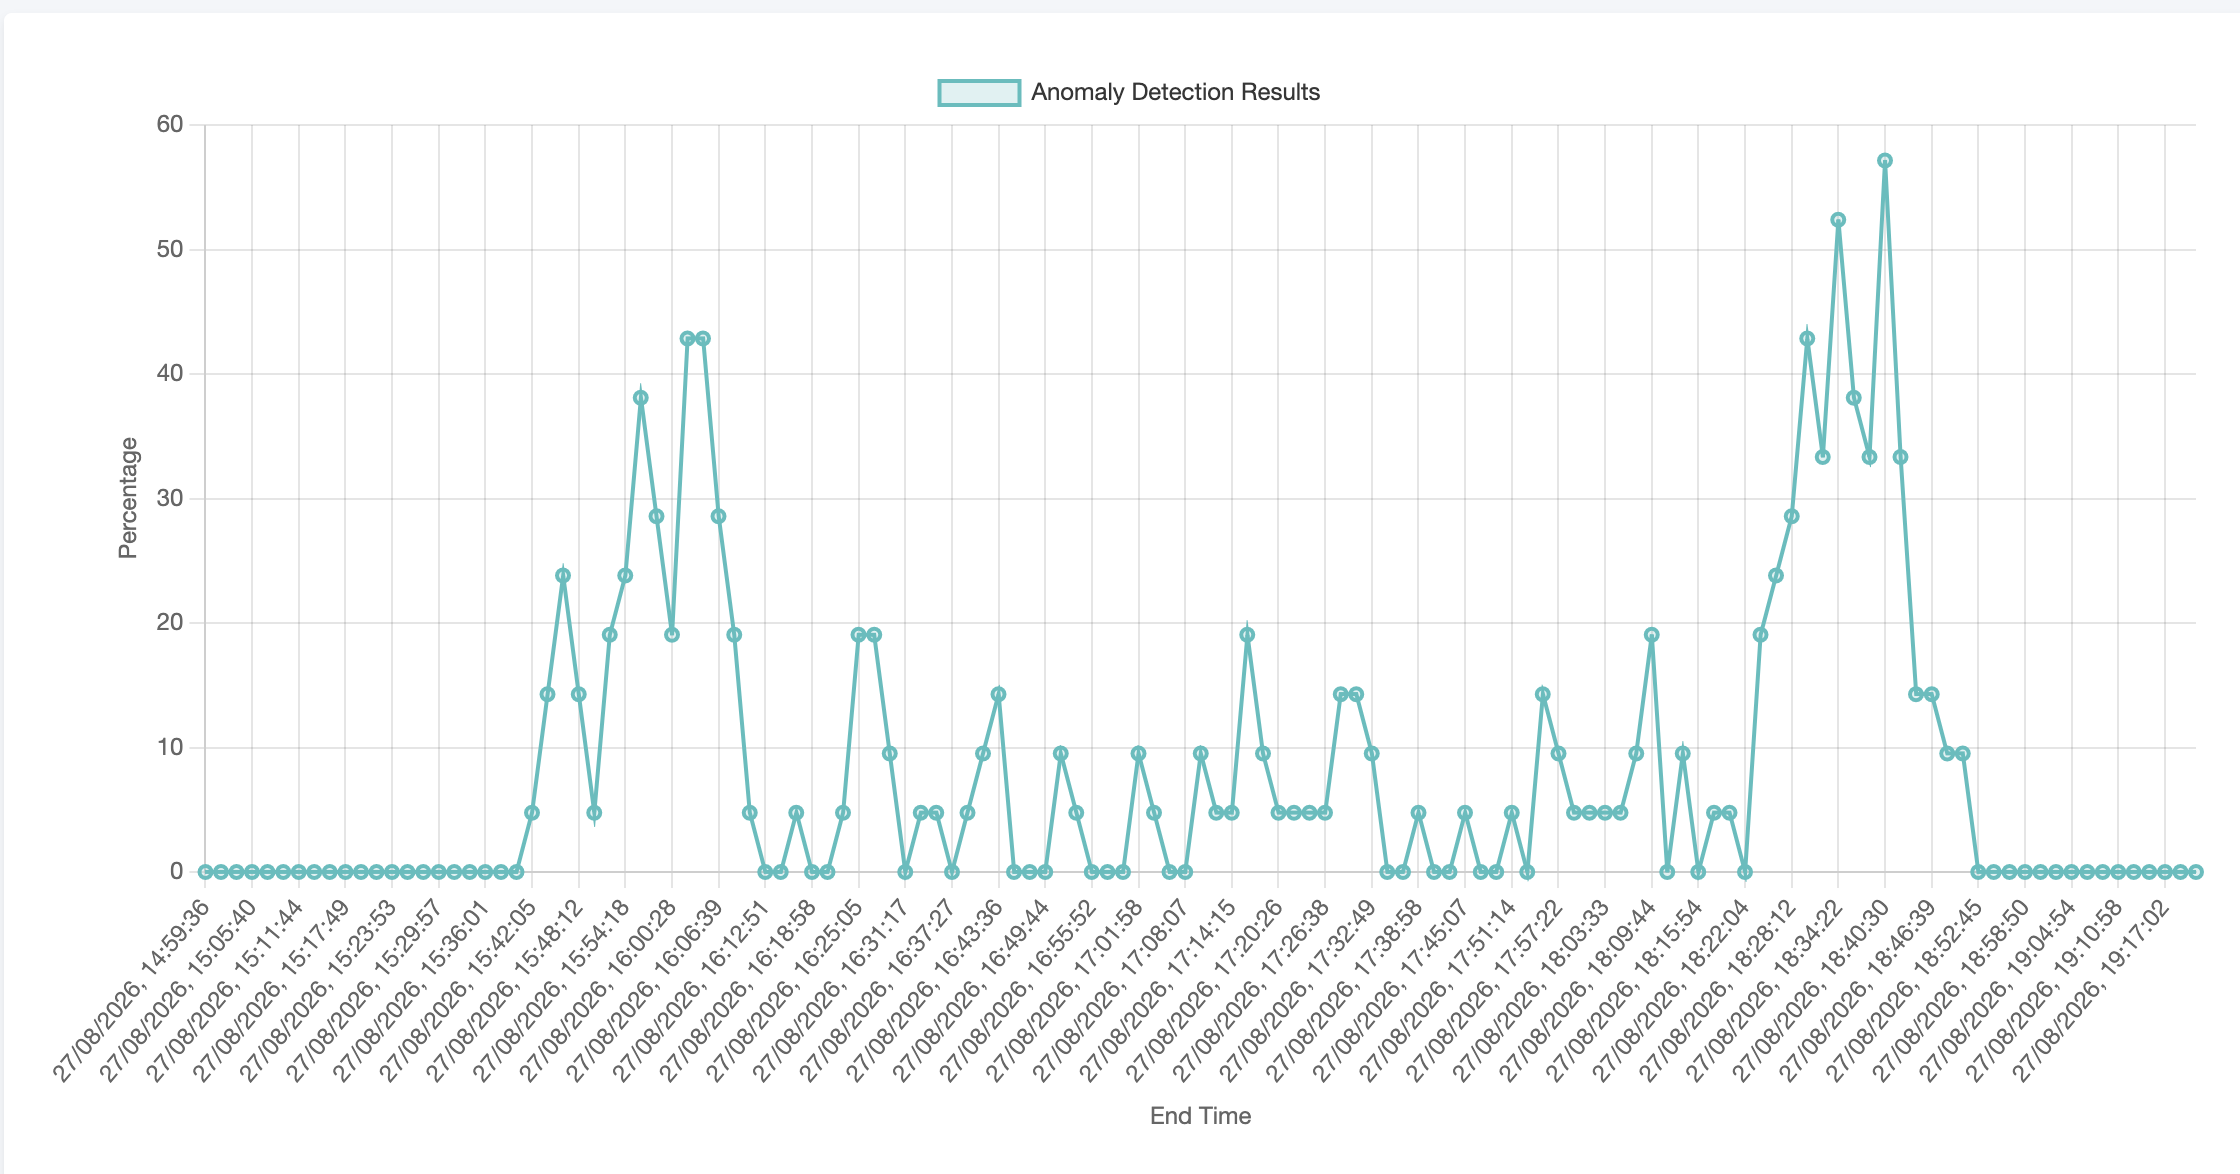
\includegraphics[width=\textwidth]{figures/boutique/scenario2/scenario2_graph_result.png}
    \caption{CloudSentinel live-monitoring view during sequential CPU stress on five Online Boutique services. The graph displays the percentage of scoreable timestamps classified as anomalous in each monitoring iteration.}
    \label{fig:multipod-livemonitoring-cpu-live}
\end{figure}

The repeated dips are consistent with the forecasting-based design of the detector. At the beginning of a sustained stress period, the lookback context mainly contains normal behaviour. The following high CPU values can then be difficult to predict, producing high prediction errors and anomaly scores. Later in the same stress period, the lookback context increasingly contains already stressed observations. A stable high-CPU state may become easier to predict from this recent context, even though it remains operationally abnormal.

CloudSentinel is not retrained during the scenario. However, the input context changes as the monitoring window moves forward. When CPU stress is removed, the reverse transition can again be difficult to predict because the recent context still contains stressed observations. This explanation is consistent with the observed graph, but the experiment does not isolate forecasting behaviour from other factors.

The effect may be compounded by the per-window Min--Max scaling described above. Each detection-only request fits a new scaler to its submitted data. Consequently, absolute CPU values can be represented differently across monitoring iterations, while the saved epsilon threshold remains unchanged. This is a framework-level interpretability problem.

\subsubsection{RCA result}
RCA was first triggered at approximately 15:42 local time, with an anomaly percentage of 4.762\%. The first RCA ranking did not show a clear causal ordering of the injected services. \texttt{frontend\_cpu} ranked first, followed by \texttt{paymentservice\_cpu}, \texttt{checkoutservice\_cpu}, and several checkoutservice-related features. Other relevant metrics were ranked much lower. For example, \texttt{paymentservice\_cpu\_throttling} ranked 32nd.

The highest anomaly percentage observed during the session occurred at approximately 18:40 local time and was 57.143\%. This event also did not identify \texttt{paymentservice}, or another clearly defined initiating service, as a clear root cause. The rankings remained dispersed across multiple services and metrics.

The RCA results therefore show that the framework can trigger and produce RCA output during a distributed disturbance. They do not show that CloudSentinel reconstructed the intended injection sequence or identified one genuine causal origin.

\subsubsection{Manual replay result}

Table~\ref{tab:multipod-manual-detection-results} summarises the manual replay results for the multi-pod scenario.

\begin{table}[htbp]
    \centering
    \small
    \caption{Manual replay results for the multi-pod CPU-stress scenario.}
    \label{tab:multipod-manual-detection-results}
    \begin{tabular}{r r r r r r r r}
        \toprule
        \textbf{Aligned rows} & \textbf{TP} & \textbf{FP} & \textbf{TN} & \textbf{FN} & \textbf{Precision} & \textbf{Recall} & \textbf{F1} \\
        \midrule
        925 & 9 & 0 & 200 & 716 & 1.000 & 0.012 & 0.025 \\
        \bottomrule
    \end{tabular}
\end{table}

The manual replay contained 925 aligned timestamps, of which 725 were labelled as part of the multi-pod CPU-stress interval. Only nine of those 725 timestamps were classified as anomalous. No normal timestamps were classified as anomalous, resulting in a precision of 1.000. However, 716 fault-labelled timestamps were classified as normal, resulting in a recall of 0.012 and an F1-score of 0.025.

The high precision should not be interpreted as broad detection coverage. It reflects the absence of false positives among only nine positive predictions. Under the stored threshold and evaluated preprocessing path, the manual workflow identified a small number of distinctive timestamps but did not detect the sustained multi-pod stress period consistently.

\subsubsection{Scenario interpretation}
The multi-pod scenario produced a much stronger live response than the single-pod scenario. The live anomaly percentage reached 57.143\%, and RCA was triggered 67 times. This shows that the end-to-end workflow was responsive to a larger distributed disturbance.

At the same time, the repeated dips in the live percentage and the low recall in manual replay show that a high live percentage should not be interpreted as reliable timestamp-level detection of the full stress interval. The forecasting-based input context and the per-window scaling behaviour both limit comparability between monitoring iterations.

The RCA rankings did not identify a clear initiating component. This outcome is partly expected because the injected CPU stress was concurrent and independently applied to multiple pods. The scenario is therefore evidence of workflow behaviour and RCA interpretability under distributed stress, rather than a valid causal-chain benchmark.

\subsection{Cross-scenario workflow summary}
Table~\ref{tab:online_boutique_workflow_summary} summarises the evidence from the two completed scenarios.

\begin{table}[htbp]
    \centering
    \small
    \caption{Cross-scenario workflow summary for Online Boutique.}
    \label{tab:online_boutique_workflow_summary}
    \begin{tabular}{p{0.18\textwidth} p{0.20\textwidth} p{0.15\textwidth} p{0.20\textwidth} p{0.20\textwidth}}
        \toprule
        \textbf{Scenario} & \textbf{Anomaly percentage observed} & \textbf{RCA triggered} & \textbf{Intervention target represented} & \textbf{Interpretation} \\
        \midrule
        Single-pod CPU stress & Yes; percentage increased and crossed the threshold, with an unexplained dip. & Yes; 9 times & Partly; paymentservice-related metrics appeared, but inconsistently. & End-to-end workflow was functional, but localisation was unreliable. \\
        Sequential multi-pod CPU stress & Yes; stronger response, with a maximum of 57.143\%. & Yes; 67 times & Partly; affected and related metrics appeared, but rankings were dispersed. & Framework responded to distributed stress, but output did not identify a clear causal origin. \\
        \bottomrule
    \end{tabular}
\end{table}

\section{Framework limitations revealed by Online Boutique}
The Online Boutique case revealed limitations that are relevant beyond the two individual scenarios. These findings concern the consistency and usability of the framework workflow, rather than only the output of the embedded algorithms.

\subsection{Preprocessing and threshold consistency}
\label{sec:preprocessing_threshold_consistency}
CloudSentinel uses different scaling behaviour in training and detection-only workflows. During training, a Min--Max scaler is fitted to the training data and used for the supplied test data. During a detection-only request, a new scaler is fitted to the submitted data. Live monitoring repeatedly submits recent data windows, so the scaling range can change between monitoring iterations.

The model's stored epsilon threshold was derived under the training-time scaling regime. Reusing that threshold with differently scaled input can make the resulting anomaly decisions difficult to compare. This helps explain why sustained CPU stress could produce high percentages at the beginning and end of a fault period but lower percentages during the middle of the same period. It also prevents direct interpretation of the manual replay metrics as validation of the live-monitoring graph.

\subsection{Configuration propagation and reproducibility}
The live-monitoring workflow required additional manual work after model training and interface configuration. In particular, configuration changes did not always propagate automatically to the components that performed monitoring or inference. Model artefacts and environment-specific settings also required manual handling.

These issues make it difficult to reproduce a successful run from the interface configuration alone. A reproducible workflow should preserve the relevant model, preprocessing settings, metric mapping, and monitoring configuration as one consistent deployment state.

\subsection{Manual data engineering and application coupling}
Online Boutique could not be connected to CloudSentinel without application-specific metric selection, Prometheus exports, timestamp alignment, reshaping, and label construction. The original datasets and examples did not provide a direct template for the new application.

This work is acceptable for a controlled research prototype, but it is a barrier to routine adoption. It also shows that CloudSentinel is coupled to assumptions about input metrics, entity names, and data format. The framework could be made more portable through declarative metric mappings, reusable preprocessing, and more automated dataset construction.

\subsection{RCA interpretability and fragmented operator workflow}
CloudSentinel and Grafana supported different parts of the diagnostic workflow. Grafana was used to inspect raw metrics and verify the effect of fault injections, while CloudSentinel presented anomaly percentages and RCA rankings. The connection between these views was limited. Users had to manually relate a CloudSentinel result to the relevant service, metric, time period, and system behaviour in Grafana.

The live-monitoring interface itself provided limited context. It displayed a graph with a percentage-based anomaly indication, but did not clearly explain what the percentage represented, which timestamps were included in the current monitoring iteration, which metrics contributed to the result, or how the configured threshold should be interpreted. The session timestamp also appeared offset from the actual execution time. As a result, a user could observe that the percentage changed without being able to directly understand why.

RCA output added limited context to this view. It was primarily expressed as ranked metrics rather than as an explanation of the affected service and likely operational cause. The rankings could contain affected metrics, but did not consistently identify the affected service or explain why a metric was considered relevant. This reduced the direct usefulness of the output for an operator.

\subsection{Implications for portability and extensibility}
The baseline evaluation shows that CloudSentinel can be adapted to Online Boutique, but that adaptation is not lightweight. Portability is limited by manual environment-specific configuration and a Prometheus-centred data path. A direct dependency on Prometheus may also limit use in environments that primarily use other observability backends; this latter limitation was not evaluated empirically in the present study.

The evaluation also does not demonstrate that analytics components can be replaced or extended easily. The observed coupling between metric preparation, model inputs, trained artefacts, thresholds, and monitoring configuration suggests that a clearer component interface and explicit data contracts would be required before pluggability can be claimed.

\section{Resource-overhead observations}
[TODO]
% C5 remains preliminary. The baseline evaluation was conducted in a constrained local Minikube cluster, but no systematic comparison of CloudSentinel CPU and memory use during idle and active operation was completed. The available observations are insufficient to support a reliable quantitative overhead claim.

% A focused idle-versus-active CPU and memory measurement can be added after the baseline evaluation is completed. Until then, resource efficiency is treated as a design requirement and as a limitation of the current evidence rather than as a completed result.

\section{NaaVRE portability case}
\label{sec:naavre_results}

NaaVRE was evaluated only after the redesigned workflow and the evaluation-only Grafana adapter existed. It is therefore not part of the original-framework baseline in this chapter. Its protocol is described in Section~\ref{sec:naavre_protocol} and its results are reported with the redesigned workflow in Chapter~9.

\section{Result summary and evidence boundary}
Table~\ref{tab:baseline_evidence_summary} makes the baseline evidence boundary explicit. Online Boutique is the controlled baseline case. The later RCAEval and NaaVRE cases evaluate the redesigned workflow and are therefore kept outside this table.

\begin{table}[htbp]
    \centering
    \small
    \caption{Completed baseline evidence and its scope.}
    \label{tab:baseline_evidence_summary}
    \begin{tabular}{p{0.20\textwidth} p{0.25\textwidth} p{0.22\textwidth} p{0.25\textwidth}}
        \toprule
        \textbf{Case} & \textbf{Evidence completed} & \textbf{Criteria supported} & \textbf{Evidence boundary} \\
        \midrule
        Online Boutique & Onboarding, two controlled CPU-stress scenarios, live workflow observations, RCA output, and manual replay. & C1--C4; preliminary C5. & Controlled local proof of concept; not a broad algorithm benchmark or production deployment. \\
        \bottomrule
    \end{tabular}
\end{table}

The Online Boutique results show that CloudSentinel can be connected to a new Kubernetes microservice application and can execute an end-to-end anomaly detection and RCA workflow. At the same time, the case reveals substantial manual onboarding effort, inconsistent preprocessing and configuration behaviour, and limited operator-oriented interpretation of the live-monitoring and RCA output. Chapter~8 evaluates these findings against C1--C5 and derives design requirements for an improvement to the framework.
